\documentclass[twoside]{article}
\input{ISC18-english.sty}
%%%%%%  Make sure to compile twice for proper cross-references. %%%%%
%%%%%% For proper display of references, compile the document twice. %%% 
\usepackage{subcaption}

\usepackage{pgfplots}

%=========== Theorem Environments ============
\theoremstyle{plain}
\newtheorem{theorem}{Theorem}[section]
\newtheorem{lemma}[theorem]{Lemma}
\newtheorem{proposition}[theorem]{Proposition}
\newtheorem{corollary}[theorem]{Corollary}
\theoremstyle{definition}
\newtheorem{definition}[theorem]{Definition}
\newtheorem{remark}[theorem]{Remark}
% ===========End of  Theorem Environments=========
% ========== Figures (TikZ/pgfplots) ============== 
\usepackage{tikz}
\usepackage{pgfplots}
\pgfplotsset{compat=1.18}
%=========Enf of Figures (TikZ/pgfplots)============
%===== Stable unit-peak Beta shape (no huge constants)=====
\pgfmathdeclarefunction{betaunit}{3}{% 
\pgfmathsetmacro{\xa}{max(min(#1,0.999999),0.000001)}%
\pgfmathsetmacro{\am}{#2-1} 
\pgfmathsetmacro{\bm}{#3-1} 
\pgfmathsetmacro{\den}{\am+\bm} 
\pgfmathsetmacro{\xmode}{\am/(\den)} 
\pgfmathsetmacro{\num}{(\xa^\am)*((1-\xa)^\bm)} 
\pgfmathsetmacro{\peak}{(\xmode^\am)*((1-\xmode)^\bm)} 
\pgfmathparse{\num/\peak} 
}
%==End of Stable unit-peak Beta shape (no huge constants)=====
% \setlength{\parindent}{5pt}    %

 \begin{document} 
\thispagestyle{empty}

\fancyhead[LE]{Bayesian Estiomation in Mixed System}

\fancyhead[RO]{Ganji and Gharari}

\begin{center}
{
\includegraphics [height=25mm, width=150.3mm] {Images/isc18E}} \\
\vspace*{-1.8cm}

\vspace*{4cm}
{\Large \bf  Bayesian Inference and Tracking of System Reliability} } \\

{\bf 
Masoud Ganji$^1${\footnote{{\bf Corresponding Author:} {\tt mganji@uma.ac.ir }}}, Fatemeh Gharari$^2$} \\
$^1,^2$ University of Mohaghegh Ardabili }
\end{center}
\rule{\textwidth}{0.2mm}   %The line upper the Abstract

\noindent{\bf Abstract:} \\
This paper develops an extended Bayesian framework for estimating and tracking system reliability with a clear focus on sequential use of data and prior information. Within this framework, we establish new theoretical results, including the uniqueness of Beta priors under moment matching, bounds for series–parallel system reliability, asymptotic normality of posterior distributions, and Bayesian consistency. We further derive limit theorems for posterior mean convergence rates and credible-interval bounds for mixed systems. Numerical examples and sequential updating schemes demonstrate how the proposed framework can be applied in practice. Overall, the approach provides a rigorous, computationally light, and reproducible methodology for reliability analysis.

\noindent{\bf Keywords:} 
Bayesian Inference, System Reliability, Posterior Consistency, Credible Bounds. 
\noindent{\bf Mathematics Subject Classification (2020):} $\rm 62F15$, $\rm 62N05$, $\rm 62P30$, $\rm 93B30$.

% \hspace{1cm}\rule{\textwidth}{0.2mm}   %The line upper the Introduction with 1 cm space
\section{Introduction}
Reliability analysis quantifies the probability that a system performs its intended function without failure over a specified mission time. Modern engineering systems often consist of multiple interdependent components arranged in series, parallel, or mixed configurations, which makes system‑level reliability inference mathematically and computationally challenging \cite{Barlow:Proschan:1996}.
Bayesian methods provide a coherent framework for reliability analysis by enabling (i) the integration of prior knowledge with observed data, (ii) full uncertainty quantification through posterior distributions, and (iii) sequential updating as new information becomes available—an essential feature for time‑evolving or continuously monitored systems. From a probabilistic standpoint, reliability modeling is deeply connected to stochastic processes and lifetime distributions, as discussed in classical probability texts such as \cite{Ross:2019}.
A wide range of studies has advanced Bayesian reliability methodology. For example, \cite{Ganji:Gharari:2016} investigated Bayesian estimation for discrete Weibull models, \cite{Abravesh:et.al.:2018} analyzed stress–strength reliability under censoring schemes, and \cite{Ganji:Mostafayi:2019} examined Bayesian change‑point detection in mixture models. Despite these contributions, there remains a lack of rigorous theoretical development that formally links Bayesian posterior inference to classical system‑reliability structures such as series, parallel, and mixed systems \cite{Barlow:Proschan:1996,Gelman:2013}.
Recent research continues to expand Bayesian reliability analysis in several directions. Refined Bayesian quadrature methods have been developed for estimating extremely small failure probabilities in complex systems \cite{Refined2024}. Updated methodological reviews highlight modern computational strategies for system‑level posterior inference and emphasize the need for theoretically grounded Bayesian reliability tools \cite{Liu2019}. Dependence modeling has also received increased attention, including copula‑based Bayesian reliability for parallel systems \cite{Lin2021} and Bayesian stress–strength analysis for series–parallel structures \cite{Zhang2025}. In addition, quasi‑Bayesian active‑learning approaches have been proposed for structural reliability problems involving rare events \cite{QuasiBayes2024}. These recent developments underscore the growing interest in Bayesian reliability but also highlight the need for a unified theoretical foundation that connects posterior inference with system‑level reliability structures.
This paper addresses this gap by establishing new theoretical results that clarify how Bayesian posterior inference at the component level translates into system‑level reliability measures.
The main purpose of this paper is to develop a unified theoretical Bayesian framework for reliability analysis of multi‑component systems. We derive new theorems that connect posterior distributions of component lifetimes with the reliability of series, parallel, and mixed systems, thereby providing a rigorous foundation for understanding how uncertainty propagates from components to the overall system.
%End new part
\section{Preliminaries}
We briefly recall standard system--reliability structures.
\noindent
\textbf{Series system.}
When all components must function for the system to succeed, the reliability is
\begin{equation}
R_{\text{series}} = \prod_{i=1}^{n} R_i .
\end{equation}
\noindent
\textbf{Parallel system.}
When the system functions as long as at least one component works, reliability is
\begin{equation}
R_{\text{parallel}} = 1 - \prod_{i=1}^{n} (1 - R_i).
\end{equation}
\noindent
\textbf{Mixed system (example).}
If components 1 and 2 are in series, and component 3 is in parallel with that series pair, the system reliability is
\begin{equation}
R_{\text{mix}} = R_1 R_2 + R_3 - R_1 R_2 R_3 .
\end{equation}
\medskip
If the mean $\mu$ and variance $v$ of a component reliability $R$ are known, the parameters of a Beta distribution obtained by moment matching are
$$
s = \frac{\mu(1-\mu)}{v} - 1, \qquad 
\alpha = \mu s, \qquad 
\beta = (1-\mu)s .
$$
Posterior updating with Binomial data $x \sim \text{Binomial}(n,R)$ yields
\begin{equation}
R \mid x \sim \text{Beta}(\alpha + x,\; \beta + n - x).
\end{equation}

\section{Main Results}

We now present several theoretical results that extend the Bayesian reliability framework. 
The first theorem establishes the uniqueness of the Beta prior obtained via moment matching.

\begin{theorem}[Uniqueness of Beta Prior via Moment Matching]
Let $\mu$ and $v$ be the mean and variance of the system reliability, with 
$0 < \mu < 1$ and $0 < v < \mu(1-\mu)$. 
Then the Beta distribution parameters $(\alpha,\beta)$ obtained from
$$
s = \frac{\mu(1-\mu)}{v} - 1,\qquad 
\alpha = \mu s, \qquad 
\beta = (1-\mu)s,
$$
are uniquely determined and positive.
\end{theorem}

The next two theorems provide bounds for system reliability and establish the asymptotic normality of the posterior distribution.

\begin{theorem}[Bounds for System Reliability]
Consider a system of independent components with reliabilities $R_i$.  
If $R_i \sim \text{Beta}(\alpha_i,\beta_i)$, then the system reliability satisfies
\begin{equation}
\prod_{i=1}^n \mathbb{E}[R_i] 
\;\leq\; \mathbb{E}[R_{\text{series}}] 
\;\leq\; \min_i \mathbb{E}[R_i],
\end{equation}
\begin{equation}
\max_i \mathbb{E}[R_i] 
\;\leq\; \mathbb{E}[R_{\text{parallel}}] 
\;\leq\; 1 - \prod_{i=1}^n (1 - \mathbb{E}[R_i]).
\end{equation}
\end{theorem}

\begin{theorem}[Asymptotic Normality of the Posterior]
Suppose $R \sim \text{Beta}(\alpha,\beta)$ and $X \sim \text{Binomial}(n,p)$.  
Then the posterior distribution
\begin{equation}
R \mid X \sim \text{Beta}(\alpha + X,\; \beta + n - X)
\end{equation}
satisfies, as $n \to \infty$,
\begin{equation}
\sqrt{n}\left(R - \frac{X}{n}\right)
\;\overset{d}{\longrightarrow}\;
\mathcal{N}\!\left(0,\; p(1-p)\right).
\end{equation}
\end{theorem}

We now investigate Bayesian consistency, the rate of posterior mean convergence, and credible interval bounds for mixed systems.

\begin{theorem}[Bayesian Consistency]
Let the true system reliability be $p_0 \in (0,1)$.  
If the prior distribution for $R$ has full support on $(0,1)$, then for any $\epsilon > 0$,
\begin{equation}
\Pr\!\left(|R - p_0| > \epsilon \,\big|\, \text{data}\right)
\;\longrightarrow\; 0
\qquad \text{as } n \to \infty.
\end{equation}
\end{theorem}

\begin{theorem}[Rate of Posterior Mean Convergence]
Let $\hat{R}_n = \mathbb{E}[R \mid \text{data}]$. Then
\begin{equation}
\sqrt{n}(\hat{R}_n - p_0)
\;\overset{d}{\longrightarrow}\;
\mathcal{N}(0,\, p_0(1-p_0)).
\end{equation}
\end{theorem}

\begin{theorem}[Credible Interval Bounds for Mixed Systems]
For a mixed system $R_{\text{mix}}$ with Beta priors on components,  
any $(1-\gamma)$ Bayesian credible interval $C_\gamma$ satisfies
\begin{equation}
\Pr(R_{\text{mix}} \in C_\gamma \mid \text{data}) \;\geq\; 1-\gamma,
\end{equation}
and its width admits the upper bound
\begin{equation}
\text{Length}(C_\gamma) \leq K\, n^{-1/2},
\end{equation}
for some constant $K>0$ depending only on the true reliability $p_0$.
\end{theorem}

\section{Illustrative Examples}

\noindent
\textbf{Component Priors.}
Choose independent priors:
\begin{equation}
R_1 \sim \mathrm{Beta}(6,2), \qquad
R_2 \sim \mathrm{Beta}(7,3), \qquad
R_3 \sim \mathrm{Beta}(8,2).
\end{equation}
\noindent
Moment matching for the mixed system reliability $R_{\text{mix}}$ yields
\begin{equation}
R_{\text{mix}} \sim \mathrm{Beta}(22,4).
\end{equation}
\noindent
\textbf{Small-Sample Posterior.}
Figure~\ref{fig:small-sample} compares the prior and posterior distributions of the
reliability parameter $R$ for a small sample size.  
The prior distribution $\mathrm{Beta}(22,4)$ (dashed) is updated to the posterior
\begin{equation}
R \mid (n=20, x=3) \sim \mathrm{Beta}(39,7),
\end{equation}
based on $n=20$ observations with $x=3$.  
The shift and narrowing of the posterior density illustrate the refinement of uncertainty
through Bayesian updating.

\begin{figure}[h!]
\centering
\begin{tikzpicture}
\begin{axis}[
    width=0.85\linewidth,
    height=5.5cm,
    xlabel={$R$},
    ylabel={Relative density},
    xmin=0.6, xmax=1.0,
    ymin=0, ymax=1.5,
    legend style={at={(0.97,0.97)},anchor=north east},
    grid=both,
    unbounded coords=discard,
    restrict x to domain=0.600001:0.999999,
    restrict y to domain=0:5,
    filter discard warning=false
]
% Prior dashed
\addplot[thick,dashed,domain=0.6:1,samples=400] { betaunit(x,22,4) };
\addlegendentry{Prior Beta(22,4)}
% Posterior solid
\addplot[thick,solid,domain=0.6:1,samples=400] { betaunit(x,39,7) };
\addlegendentry{Posterior Beta(39,7)}
\end{axis}
\end{tikzpicture}
\caption{Prior (dashed) vs.\ posterior (solid), $n=20$, $x=3$.}
\label{fig:small-sample}
\end{figure}
\noindent
\textbf{Large-Sample Posterior.}
Figure~\ref{fig:large-sample} compares the prior and posterior distributions of $R$
for a larger sample size.  
The prior $\mathrm{Beta}(22,4)$ (dashed) is updated to the posterior
\begin{equation}
R \mid (n=100, x=15) \sim \mathrm{Beta}(107,19),
\end{equation}
based on $n=100$ observations with $x=15$.  
Compared with the small-sample case, the posterior is more concentrated, reflecting
reduced uncertainty and the stronger influence of the observed data.

\begin{figure}[h!]
\centering
\begin{tikzpicture}
\begin{axis}[
    width=0.85\linewidth,
    height=5.5cm,
    xlabel={$R$},
    ylabel={Relative density},
    xmin=0.6, xmax=1.0,
    ymin=0, ymax=1.5,
    legend style={at={(0.97,0.97)},anchor=north east},
    grid=both,
    unbounded coords=discard,
    restrict x to domain=0.600001:0.999999,
    restrict y to domain=0:5,
    filter discard warning=false
]
% Prior dashed
\addplot[thick,dashed,domain=0.6:1,samples=400] { betaunit(x,22,4) };
\addlegendentry{Prior Beta(22,4)}
% Posterior solid
\addplot[thick,solid,domain=0.6:1,samples=400] { betaunit(x,107,19) };
\addlegendentry{Posterior Beta(107,19)}
\end{axis}
\end{tikzpicture}
\caption{Prior (dashed) vs.\ posterior (solid), $n=100$, $x=15$.}
\label{fig:large-sample}
\end{figure}

Figures~\ref{fig:small-sample} and~\ref{fig:large-sample} together illustrate the effect of Bayesian updating on the reliability distribution as the sample size increases. In both cases, the prior distribution $\mathrm{Beta}(22,4)$ represents the initial belief about the system reliability. For the small-sample case ($n=20$, $x=3$), the posterior $\mathrm{Beta}(39,7)$ shifts moderately from the prior and becomes only slightly more concentrated, indicating that limited data provide partial information and the prior still exerts noticeable influence. In contrast, for the larger sample ($n=100$, $x=15$), the posterior $\mathrm{Beta}(107,19)$ is substantially more concentrated and centered closer to the empirical reliability, reflecting reduced uncertainty and the dominance of observed data. Taken together, the figures demonstrate the Bayesian learning mechanism: as the amount of data increases, posterior distributions become more sharply peaked and increasingly data-driven, yielding greater confidence in the estimated reliability.


\section{Sequential Updating}

We consider four sequential periods of data:
\begin{equation}
(20,3), \quad (20,4), \quad (25,2), \quad (25,5),
\end{equation}
where each pair denotes $(n,x)$, the number of observations and the number of failures.

\noindent
Starting from the prior $\mathrm{Beta}(22,4)$, the posterior parameters evolve as
\begin{equation}
(22,4) \;\to\; (39,7) \;\to\; (55,11) \;\to\; (78,13) \;\to\; (98,18).
\end{equation}

\noindent
The corresponding posterior means are
\begin{equation}
0.846,\quad 0.848,\quad 0.833,\quad 0.857,\quad 0.845.
\end{equation}

\begin{figure}[h!]
\centering
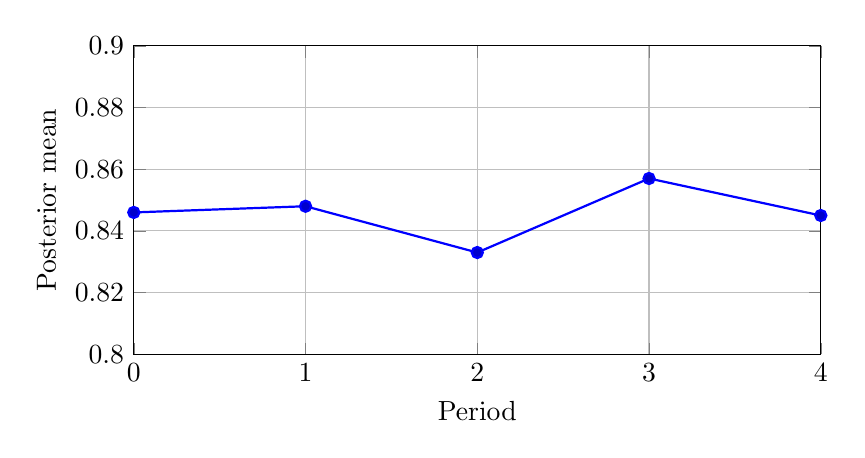
\begin{tikzpicture}
\begin{axis}[
    width=0.85\linewidth,
    height=5.5cm,
    xlabel={Period},
    ylabel={Posterior mean},
    xmin=0, xmax=4,
    ymin=0.80, ymax=0.90,
    xtick={0,1,2,3,4},
    grid=both
]
\addplot+[thick,mark=*] coordinates{
    (0,0.846)
    (1,0.848)
    (2,0.833)
    (3,0.857)
    (4,0.845)
};
\end{axis}
\end{tikzpicture}
\caption{Posterior mean reliability across sequential updates.}
\label{fig:seq-update}
\end{figure}

\paragraph{Interpretation.}
Figure~\ref{fig:seq-update} illustrates the evolution of the posterior mean reliability across four sequential updates. Although each new batch of data slightly shifts the posterior mean, the overall trajectory remains stable, fluctuating within a narrow range between $0.833$ and $0.857$. This stability indicates that the Bayesian updating procedure is not overly sensitive to individual data batches and that the accumulated evidence leads to a robust and consistent estimate of system reliability. The figure highlights how sequential Bayesian learning incorporates new information while maintaining coherence with prior and previously observed data.
%End new part
\section{Discussion and Conclusion}
We have established several theoretical results that strengthen the foundations of Bayesian reliability inference. 
Our findings show that Beta priors are uniquely determined under moment matching, 
that credible bounds for system reliability can be rigorously quantified, 
and that Bayesian estimators exhibit both asymptotic normality and consistency. 
Together, these results bridge the gap between practical computational methods and the underlying theoretical structure, 
providing a coherent and robust framework for engineers and statisticians working with reliability data.

The illustrative examples demonstrate how Bayesian updating behaves under small and large samples, 
and how sequential learning stabilizes reliability estimates over time. 
These examples highlight the practical relevance of the theoretical results and show how uncertainty is progressively reduced as more information becomes available.

Future research directions include the study of non-conjugate priors, 
the incorporation of dependence structures among components, 
and the extension of the framework to high-dimensional or network-based system reliability models. 
Such developments would further enhance the applicability of Bayesian methods to modern engineering systems, 
where complexity and interdependence play increasingly central roles.


\section*{Acknowledgments}
The authors would like to express their sincere gratitude to the reviewers for their constructive comments and suggestions, which have significantly improved the quality and clarity of this paper.

%\newpage

 \begin{thebibliography}{9}
\bibitem[Abravesh et.al.(2018)]{Abravesh:et.al.:2018} 
Abravesh A., Ganji M., Mostafaiy B. 2018, Classical and Bayesian Estimation of Stress-Strength Reliability in Type-II Censored Pareto Distributions. 
{\it Communications in Statistics - Theory and Methods}, 47, 1, 27-46. doi:10.1080/03610918.2018.1457688.}

\bibitem[Barlow and Proschan(1996)]{Barlow:Proschan:1996}
Barlow R. E. and Proschan F.  (1996), Mathematical Theory of Reliability.{\it  SIAM.}

\bibitem[Ganji  and Gharari(2016)]{Ganji:Gharari:2016} 
Ganji M. and Gharari F. (2016), Bayesian Estimation in Delta and Nabla Discrete Weibull Distributions. 
{\it Journal of Probability and Statistics}, Article ID 1969701.}

\bibitem[Ganji  and Mostafay(2019)]{Ganji:Mostafayi:2019} 
Ganji M. and Mostafay R. (2019), Bayes and Non-Bayes Estimation of Change Point in Non-Standard Mixture Inverse Weibull Distribution. 
{\it Journal of Statistical Theory and Applications}, 18,1, 79–86.}

\bibitem[Gelman  et al.(2013)]{Gelman:2013} 
Gelman, A., Carlin, J.B., Stern, H.S. and Rubin, D.B., (2013),  Bayesian Data Analysis , {\it 3rd ed. CRC Press.}

\bibitem[Ross(2019)]{Ross:2019} 
Ross S. M. (2019), Introduction to Probability Models,{\it 12th ed. Academic Press.}

\bibitem[Dang  et al.(2024)]{QuasiBayes2024}
Dang, C., Cicirello, A., Valdebenito, M.A., Faes, M.G., Wei, P. and Beer, M., 2024. Structural reliability analysis with extremely small failure probabilities: A quasi-Bayesian active learning method. {\it Probabilistic Engineering Mechanics}, 76, p.103613.

\bibitem[Zhang and Yan(2025)]{Zhang2025}
Zhang, L., Yan, R. and Wang, J., 2025. Bayesian inference for dependent stress–strength reliability of series–parallel system based on copula. {\it Scientific Reports}, 15(1), p.29504.

\bibitem[Lin et al.(2021)]{Lin2021}
Lin C.H. and Huang Y. (2021), Copula-based Bayesian reliability analysis of a product of a probability and a frequency model for parallel systems when components are dependent.
{\it Applied Sciences}, 11(4), 1697.

\bibitem[Liu and Abeyratne(2019)]{Liu2019}
Liu, Y. and Abeyratne, A.I., 2019. Practical applications of Bayesian reliability. {\it John Wiley & Sons}.

\bibitem[Wang et al.(2024)]{Refined2024}
Wang, L., Hu, Z., Dang, C. and Beer, M., 2024.
 Refined parallel adaptive Bayesian quadrature for estimating small failure probabilities.}
 {\it Reliability Engineering & System Safety}, 244, p.109953.

\end{thebibliography}
\end{document}


